% プロジェクト学習中間報告書書式テンプレート ver.1.0 (iso-2022-jp)

% 両面印刷する場合は `openany' を削除する
\documentclass[openany,11pt,papersize]{jsbook}

% 報告書提出用スタイルファイル
%\usepackage[final]{funpro}%最終報告書
\usepackage[middle]{funpro}%中間報告書

% 画像ファイル (EPS, EPDF, PNG) を読み込むために
\usepackage[dvipdfmx]{graphicx,color}

%数式の表示に利用するため
\usepackage{amsmath,amssymb}

%アルゴリズムの表示に利用するパッケージ
\usepackage{algorithm}
\usepackage{algorithmic}

%枠をつけるためのパッケージ
\usepackage{ascmac}

%図の位置調整パッケージ
\usepackage{here}

\usepackage{listings}
% ここから -->
\usepackage{calc,ifthen}
\newcounter{hoge}
\newcommand{\fake}[1]{\whiledo{\thehoge<70}{#1\stepcounter{hoge}}%
  \setcounter{hoge}{0}}
% <-- ここまで 削除してもよい


% 年度の指定
\thisYear{2017}

% プロジェクト名
\jProjectName{FUN-ECM プロジェクト}

% [簡易版のプロジェクト名]{正式なプロジェクト名}
% 欧文のプロジェクト名が極端に長い(2行を超える)場合は,短い記述を
% 任意引数として渡す.
%\eProjectName[Making Delicious curry]{How to make delicious curry of Hakodate}
\eProjectName{FUN-ECM Project}


% <プロジェクト番号>-<グループ名>
\ProjectNumber{11-A}

% グループ名
\jGroupName{Aグループ}
\eGroupName{A Group}

% プロジェクトリーダ
\ProjectLeader{1015014}{中島俊平}{Shunpei Nakajima}

% グループリーダ
\GroupLeader  {1015014}{中島俊平}{Shunpei Nakajima}

% メンバー数
\SumOfMembers{8}
% グループメンバ
\GroupMember  {1}{1015014}{中島俊平}{Shunpei Nakajima}
\GroupMember  {2}{1015082}{福永慧}{Kei Fukunaga}
\GroupMember  {3}{1015112}{小澤貴也}{Takaya Ozawa}
\GroupMember  {4}{1015182}{落合航平}{Kouhei Otiai}
\GroupMember  {5}{1015195}{広瀬大樹}{Taiki Hirose}
\GroupMember  {6}{1015202}{金子真澄}{Masumi Kaneko}
\GroupMember  {7}{1015237}{水上敬介}{Keisuke Mizukami}
\GroupMember  {8}{1015260}{外山拓}{Taku Toyama}

% 指導教員
\jadvisor{白勢政明,由良文孝}
% 複数人数いる場合はカンマ(,)で区切る.カンマの前後に空白は入れない.
\eadvisor{Masaaki Shirase, Fumitaka Yura}

% 論文提出日
\jdate{2017年7月26日}
\edate{July~26, 2017}

\begin{document}
%
% 表紙
\maketitle

%前付け
\frontmatter

% 和文概要
\begin{jabstract}

 私達のプロジェクトの目的は,より大きな桁数の素因数を見つけることである.素因数分解が重要であることの背景として,RSA暗号がある.RSA暗号は,40年前に考案された初めての公開鍵暗号で,現在でもデジタル署名などで利用されている.RSA暗号は,「大きい桁数の2つの素数からなる合成数を素因数分解することが難しい」ということで安全が保証されているが,近年,より高い安全性を持つ楕円曲線暗号が利用されてきている.そこでFUN-ECMプロジェクトでは,楕円曲線法(ECM)を用いて,より大きい桁数の素因数分解を行うプログラムを作成し,RSA暗号の安全性について検証を行う.更に私たちは,大きい数の素因数分解をランキングしたサイトである,ECMNET\cite{EN2017}やSTUDIO KAMADA\cite{SK2017}へのランクインを目標として掲げ活動を行った.

 まず私達は,理論班とプログラム班に分かれ活動を行っている.理論班の目的は,ECMの高速化のための論文を理解し,プログラム班に引き継ぐことである.プログラム班の目的は,理論班が準備したアルゴリズムを実装し,高速化できているか確かめることである.

 理論班は,Stage2をより高速に行えるアルゴリズムの発見・理解を目標とした.昨年度のプログラムに使われていた理論の理解,Baby-step Giant-step法の理解,PARI/GPでの実装を行った.

 プログラム班は,前年度に作成された素因数分解プログラムをさらに高速化することを目標とした.昨年度のプログラムで余分に座標変換を行っていた部分のコードの修正,並列処理の強制終了の機能の追加,Baby-step Giant-step法の実装,Stage2の実行速度のテストを行った.

以上の2つの班が互いに足りない部分を補完しあい活動を行った.その結果,Stage2の高速化に成功し,素因数分解を高速に行えるプログラムが完成した.



% 和文キーワード
\begin{jkeyword}
素因数分解,楕円曲線法,ECMNET,エドワーズ曲線,拡張射影座標,RSA暗号,Baby-step Giant-step法
\end{jkeyword}
\bunseki{中島俊平}
\end{jabstract}

%英語の概要

\begin{eabstract}

~The goal of our project team is to find prime factor as large as possible. Factorizations in prime numbers have become more important because of RSA cryptosystem. RSA cryptosystem which was invented 40 years ago is still being used for digital signatures. RSA cryptosystem has been seemed to be safe because it is difficult to prime factorize a composite number composed of two prime numbers with large number of digits. However, elliptic curve cryptography has been used in recent years because it's safety is higher than RSA. Therefore, we create a program that performs prime factorization with a larger number of digits by the elliptic curve method. Then, we verify safety of the RSA cryptosystem. For that purpose, we have carried out activity with the goal of ranking in ECMNET\cite{EN2017} and STUDIO KAMADA\cite{SK2017}. ECMNET and STUDIO KAMADA is a website ranked by large number of prime factorization.

~First, we divided into two group that Theory team and Program team. The purpose of Theory team was to understand essays for ECM speed up, and to hand over it to Program team.
The purpose of Program team is to implement algorithm which prepared Theory team and to validate whether or not we can do increase in speed of program.

~The theory group aimed for algorithmic discovery and understanding to be able to perform Stage2 speed up. We understood a theory used for a program of last year, we understood Baby-step-Giant-step, we implemented PARI/GP.

~Programming group aimed to speed up the prime factorization program created in last year. We modified the code of the part where the coordinate conversion was extra last year program, implemented Baby-step Giant-step method, added the function of forcibly terminating parallel processing, and tested speed of Stage 2.

~These two groups complemented each other missing parts and carried out activities. As a result, we succeeded in speed up Stage 2, and completed a program capable of fast prime factorization.

% 英文キーワード
\begin{ekeyword}
Elliptic Curve Method, prime factorization, ECMNET, Twisted Edwards Curve, Extended Twisted Edwards Coordinates, RSA cryptosystem, Baby-step Giant-step method
\end{ekeyword}
\bunseki{中島俊平}
\end{eabstract}

\tableofcontents% 目次

\mainmatter% 本文のはじまり

\chapter{背景}

大きい桁数の素因数分解は近年重要になっている.そこで,楕円曲線法を利用し素因数分解を行い,ECMNETにランクインすることが私たちの目的である.

\bunseki{中島俊平}

\section{本プロジェクトの背景}

暗号化技術は,情報の保護やコンピュータセキュリティにおいて欠かせない技術である.ファイルの暗号化の他に,HTTPSや,無線LANにおける通信など多くの場面で暗号化技術が利用されている.しかし,暗号化技術は常に進化する攻撃方法により解読の脅威に晒されている.様々な攻撃方法から安全な暗号アルゴリズムを作成するためには,作成する側が暗号解読の方法を知る必要がある.暗号の安全性評価には暗号解読の技術が利用されていて,暗号の強度は暗号解読に必要な情報量と計算量によって評価される.今回のプロジェクトでは,その暗号解読アルゴリズムの1つである,楕円曲線法を学ぶ.\\
 現在,有名な公開鍵暗号の1つにRSA暗号がある.RSA暗号は,桁数が大きい合成数の素因数分解が困難であることを安全性の根拠とした暗号である.RSA暗号を解読する時は合成数の元となる2つの素因数を見つけ出す必要がある.ECMでは,与えられた曲線の点が無限遠点になることによって,因数が発見される.この性質を利用してRSA暗号を解読する.\\
 楕円曲線法にはStage1とStage2があり,Stage1で素因数分解できなかった場合,Stage2で素因数分解を試みる.前年度のプロジェクトではStage1のプログラムは完成していたため,今年度ではStage2の完成させることを課題とした.また,ECMNETという暗号解読した素因数の大きさを競うサイトがあり,Stage2を実装することでECMNETでのランクインをすることを目標として掲げた.

\bunseki{福永慧}

\section{ECMNETとは}

ECMNETとは,楕円曲線法を用いて解読された素因数の大きさをランキング形式で競うWebサイトである.ECMNETにランクインするためには,現在登録されている素因数よりも大きな素因数を見つける必要がある.

\bunseki{福永慧}

\section{課題の概要}\label{sec:gaiyou}

本プロジェクトでは既にStage1におけるプログラムが完成していたため,Stage2を作成する.Stage2を完成させることで,より大きな合成数を素因数分解することを目指す.また,本プロジェクトでの活動をWebサイトを用いて,FUN-ECMの情報を外部に発信する.

\bunseki{福永慧}

\chapter{到達目標}

\section{本プロジェクトにおける目的}\label{sec:mokuteki}

FUN-ECMでECMNETに記載されるためには既存のプログラムを改善し,単位時間ごとの計算速度を向上させる必要がある.そのため,この目的を達成するために2つのことを実施した.

\begin{itemize}
\item 既存のプログラムの高速化を図る
\item Stage2においての新たなアルゴリズムの実装
\end{itemize}

\bunseki{水上敬介}

\section{課題達成の為の班分け}
前年度のプロジェクトでは前期で楕円曲線法についての学習を行い,後期でアルゴリズムの提案・実装を行っていた.しかし,このような日程でプロジェクトを進行していくと以下のような問題が発生した.

\begin{itemize}
\item 実際にプログラムを実装する期間が少ない
\item 完成したプログラムを試行する期間が少ない
\item 巨大な合成数の分解を行いにくい
\end{itemize}

本プロジェクトでは,5月上旬まで全員で楕円曲線法についての基礎学習を行った.5月中旬以降,既存のプログラムを改善するためにグループ全員でアルゴリズムの理解と実装をするのは効率が悪いと判断し,プログラム班,理論班の2つのグループに班分けをした.以下にそれぞれの班の課題を述べる.

\begin{description}
 \item[理論班]\mbox{}\\ 
	    ECMについて理解を深め,Stage2での新たなアルゴリズムの発見,理解に取り組んだ.理解したアルゴリズムをプログラム班に説明した.

 \item[プログラミング班]\mbox{}\\
	    既存のプログラムの内容を理解し,プログラムの動作内容の理解に取り組んだ.理論班から提示されたアルゴリズムをもとに,既存のプログラムに実装を行った.
\end{description}
\bunseki{水上敬介}

\chapter{活動内容}

プロジェクトが発足した当初,楕円曲線についての基礎知識がなかったため,去年のプロジェクトでも基礎知識を身につけるために使われた資料を用いて,理解した.理解できないところはプロジェクトリーダーが主体となって解説をしてもらい楕円曲線についての基礎知識を学んだ.その後,アルゴリズムの提案をする理論班,提案されたアルゴリズムをプログラムに実装するプログラミング班に分けてプロジェクトを進行した.

\bunseki{水上敬介}

\section{基礎学習}

去年のプログラムを理解するために5月の中頃までメンバー全員が楕円曲線法のアルゴリズムや基礎知識についての学習を行った.具体的な内容は以下の通りである.
\begin{description}
 \item[有限体]\mbox{}\\ 
$素数pに対し,0からp-1までの整数の集合\mathbb{F}_p=\{0,1,…,p-1\}を有限体と言う.\mathbb{F}_pでは四則演算が可能であり,ECMではこの範囲で考える.$
 \item[Euclidの互除法]\mbox{}\\
$自然数a,b(a≧b)に対して以下の操作を繰り返し行い,余りが0になるまで行うことによってa,bの最大公約数を求めるものである.$

	%\begin{center}
	%	$a÷b=q1*b+r1 (q1:aをbでわった時の商,r1:aをbでわった時の余り)$
%
%		$b÷r1=q2*r1+r2 (q2:bをr1でわった時の商,r2:bをr1でわった時の余り)$
%
%		$r1÷r2=q3*r2+r3 (q1:r1をr2でわった時の商,r1:r1をr2でわった時の余り)$
%
%		$rn-2÷rn-1=qn (q2:rn-2をrn-1でわった時の商) ここで操作終了$
%	\end{center}
%
\begin{algorithm}[h]                   
\caption{Euclidean Algorithm}
\label{alg E}                          
\begin{algorithmic}                  
\REQUIRE $a,b \in \mathbb{N} , \quad a,b \neq 0,\quad a\ge b$
\ENSURE $\gcd (a,b)$
\WHILE {$b \neq 0$}
\STATE $q \leftarrow a/b$
\STATE $r \leftarrow a\mod b$
\STATE $a \leftarrow b$
\STATE $b \leftarrow r$
\ENDWHILE
\end{algorithmic}
\end{algorithm}
$以後,a,bの最大公約数を\gcd (a,b)と表記することとする.$
	
 \item[拡張Euclidの互除法]\mbox{}\\
$与えられた整数a,b,cに対し,未知数x,yに関する一次方程式ax+by=c$の整数解は,1組存在すれば無数に存在する.この方程式を一次不定方程式という.一次不定方程式の解を求めるには,拡張Euclidの互除法が有効である.拡張$Euclidの互除法は,$自然数a,bに関する一次不定方程式ax+by=gcd(a,b)を満たす無数の整数x,yを効率よく求めることができるというものである.例として174x+69y=3の整数解を求める.$
まずEuclidの互除法を用いて174と69の最大公約数を求める.$
	\begin{align*} 
		174/69&=2*69+36 \\
		69/36&=1*36+33 \\
		36/33&=1*33+3 \\
		33/3&=11 	
 	\end{align*}
	となる.そしてこれらは
	\begin{align*} 
	3&=36-33*1 \\
	33&=69-36*1 \\
	36&=174-69*2 \\
 	\end{align*}
	と表せるので
	\begin{align*} 
	3&=36-33*1 \\
	&=36-(69-36*1)*1 \\
	&=36*2+69*(-1) \\
	&=(174-69*2)*2+69*(-1) \\
	&=174*2+69*(-5)
 	\end{align*}
以上より,$174x+69y=3の整数解は(x,y)=(2,-5)$と求めることができる.
有限体$\mathbb{F}_p$において除算$a÷b$を計算する場合, $pとb$は互いに素なので, 拡張Euclidの互除法により不定方程式$px + by = 1 の解(x_0, y_0)$を求めることができる.このとき$px_0+ by_0= 1$となるので, 有限体$\mathbb{F}_p$上では$by = 1,つまりb^{−1} = y_0$が成立する.よって$a÷b=a×b^{-1}=a×y_0$と変形することで, 除算を乗算に置き換えて計算できる.


	
\item[楕円曲線の定義方程式]\mbox{}\\
$a,b \in \mathbb{F}_pに対してy^2 = x^3 + ax + bで定義される曲線を素体Fp上の楕円曲線という.$

\item[楕円曲線の加算と逆元]\mbox{}\\
$(加算) 楕円曲線上のある2点P,Qを通る直線をℓとすると,楕円曲線と直線 \ell の3つ目の交点R’(=P×Q)のx軸に関する対称点をRとする.これで得られた点RをR'の逆元と呼び,R=-R'が成り立つ.また,RをPとQを加算した点と定義し,R=P+Qが成り立つ.$

\item[無限遠点]\mbox{}\\
$楕円曲線上の点Pとその逆元-Pをとり,P+(-P)を考える.そうすると,2点を通る直線と楕円曲線にはPと-Pの他には交点が存在しない.このような状態のときに,存在しない点を仮想的に考え,それを無限遠点と呼び,P+(-P)= Oが成り立つ.$

\item[楕円曲線の2倍算]\mbox{}\\
$楕円曲線上の点Pの接線を \ell とし,楕円曲線と直線 \ell のP以外の交点をR'とし,R'の逆元をRとする.このRはR=P+P=2Pであり.楕円曲線の2倍算と定義する.$
	
\item[楕円曲線のスカラー倍算]\mbox{}\\
$点Pと自然数dに対して,点Pをd倍(dP=P+P+P+P+・・・・+P(d個の和))することを,楕円曲線のスカラー倍算という.$

\end{description}
以上のことを基礎学習として学んだ.以下の章では,2つの班のそれぞれの活動内容を記述する.

\bunseki{落合航平}

\section{理論班}
理論班では,新しいアルゴリズムを探し,プログラム班に提案した.以下は具体的内容である.

\subsection{ECMの原理の理解}
まず,私たちは,ECMを用いた素因数を求めるプロセスについて,論文を読むことで学習した.

合成数$N$について,その素因数$p$を見つけることを考える.
十分大きな自然数$n$,楕円曲線上のある点$P$に対して,$ \bmod{N} $で$ nP=(\frac{X}{Z},\frac{Y}{Z}) $を計算する.$gcd(Z,N)$により,$p$が確率的に求まる.(もしも,$Z \equiv 0 \pmod{p}$ならば,成功する)

%Stage1

ECMのStage1では,楕円曲線上のある点$P$,ある適切な自然数$B1$に対して,$2$~$B1$までの最小公倍数$L$が存在する.$\bmod{N}$で,$Q_{0}=LP$を計算する.
ここで,$LP = O\pmod{p}$が成立するとき,素因数が求まる.

%Stage2

ECMのStage2では,ある適切な自然数$B2$に対して,$B1<s<B2$を満たす全ての素数$s_{1},s_{2},...,s_{n}$について,それぞれ$s_{i}Q_{0} \ (i=1,2,...,n)$を計算する.
$sQ_{0} = O \pmod{p} $を満たす$s$が存在するとき,素因数が求まる.


\bunseki{金子真澄}

\subsection{Baby-step Giant-step法の理解}
Stage2の高速化を図るため,基礎学習で学習したBaby-step Giant-step法をプログラムに導入しようと考えた.
その際,基礎学習だけではBaby-step Giant-step法の理解が不足していたため,他の文献を探した.担当教員が紹介してくださった''Implementing the Elliptic Curve Method of Factoring in Reconfigurable Hardware''\cite{BSGS2006}という論文を深く読むことにした.


$0<a<B2$を満たすある自然数$a$,$B1<s \leq B2$を満たす素数$s$に対して,適当な自然数$v$,$u$を用いて$s$は次のように表すことができる.

\[s=av \pm u \ \ \ (0 < u < a)\]

Stage2が成功するときの条件$sQ_{0}=O (\bmod{p})$は,上式を用いて次のように変形できる.

\[sQ_{0}=O (\bmod{p}) \]
\[ \Longleftrightarrow (av \pm u)Q_{0} = O(\bmod{p})\]
\[ \Longleftrightarrow avQ_{0} = \pm uQ_{0}  \]


\begin{algorithm}[H]
\caption{Baby-step Giant-step法}\label{}
\begin{algorithmic}
\REQUIRE $N: 合成数,E: 楕円曲線,Q_{0}=kP_{0}: Stage1の結果, a,B1,B2: ある適当な自然数$

\FOR{each $i=1$ to $a-1$}
  \STATE $ H[i] \leftarrow i*Q_{0} $
\ENDFOR

\STATE $Q \leftarrow aQ_{0}$
\STATE $d \leftarrow 1$

\FOR{each prime $s = B1$ to $B2$}
  \STATE $u \leftarrow s/a$
  \STATE $v \leftarrow s\%a$
  \STATE $G \leftarrow v*Q$
  \STATE $d \leftarrow d*(G_x-H[i]_x)$
\ENDFOR

\STATE $q \leftarrow gcd(d,N) $

\IF{$q > 1$}
  \RETURN $q$
\ELSE
  \RETURN FAIL
\ENDIF
\end{algorithmic}
\end{algorithm}

さらに,私たちは,$a$の値を小さな素数の積とすること,配列$H$の要素数を減らすことを提案した.
もしも,$s=av+u$が素数であるならば,$gcd(a,u) = 1$が成り立つ.このため,配列$H$に$gcd(a,u) = 1$のときのみ$uQ_{0}$を保存するとよい.加えて,$a$が小さな素因数の積とすると,$a$と$u$が共通の因数を多く持つため,$uQ_{0}$を計算する回数が少なくなる.
PARI/GPで実装し,理論の理解を深め,プログラム班に伝えることができた.

\bunseki{金子真澄}

\subsection{Montgomery curveの導入の検討}

私たちは,昨年度のアルゴリズムを理解するため,Weierstrass型以外の形式の楕円曲線について調べ,その中でMontgomery curveを発見した.Montgomery curveは加算の一回あたりの計算量が小さいため,これを導入することでStage1の高速化が可能かどうか検討した.

Montgomery curveは,方程式
\[
By^2 = x^3 + Ax^2 + x \ \ \ s.t. \ B(A^2-4) \neq 0
\]
で定義され,Weierstrass型と同値な曲線である.

\bunseki{金子真澄}


\section{プログラミング班}
プログラム班では,昨年度のFUN-ECMプロジェクトで作成したプログラムを使用し,単位時間あたりの計算量を増幅させるために,プログラムの改善を行った.高速化するために,Stage2でのBaby-step Giant-step法の実装,去年のソースコードの不具合の修正を行った.また,昨年度のプログラムと今年度のプログラムの速度を比較するために,計測方法を確立させた.具体的には以下の通りである.

\bunseki{水上敬介}

\subsection{座標変換の際の冗長なコストの削減}\label{sec:alg1}
前年度のプロジェクトで作成されたECM プログラムでは,スカラー倍をする際の座標を射影座標から拡張射影座標に変換していた.スカラー倍を行う処理はECMプログラムを実行する際に何度も使われるので,処理速度に影響する.そのため,最初から拡張射影座標を用意することによって座標変換する分のコストを減らすことが出来た.射影座標から拡張射影座標に変換する際に使われたアルゴリズムをAlgorithm 3に示す.

\begin{algorithm}[H]                      
\caption{Projective Coordinates to Extended Coordinates}         
\label{alg1}                          
\begin{algorithmic}                  
\REQUIRE (PX,PY,PZ) is Projective, (EX,EY,ET,EZ) is Extended, $N \geq 2$
\ENSURE (EX,EY,ET,EZ)
\STATE $EX \leftarrow PX \times PZ$
\STATE $EX \leftarrow EX \bmod N$
\STATE $EY \leftarrow PY \times PZ$
\STATE $EY \leftarrow EY \bmod N$
\STATE $ET \leftarrow PX \times PY$
\STATE $ET \leftarrow ET \bmod N$
\STATE $EZ \leftarrow PZ \times PZ$
\STATE $EZ \leftarrow EZ \bmod N$
\end{algorithmic}
\end{algorithm}

Algorithm 3では,乗算を4回とmodの計算を4回行っている.プログラミング班では,スカラー倍を行う前に行われていたAlgorithm 3を省略することによって,計算コストを削減することが出来た.

\bunseki{福永慧}

\subsection{ソースコードの改善}\label{sec:alg2}
\subsubsection{scalar関数における引数の修正}

前年度のプロジェクトではスカラー倍を行うときに座標Pのみを用意して,座標Pをスカラー倍したものを座標Pに代入していた.そのため,スカラー倍の処理を複数回行った場合,スカラー倍された座標にスカラー倍を行っていたことが分かった.しかし,スカラー倍を複数回行った場合でも,1回分のスカラー倍の座標が必要であった.この問題はスカラー倍が行われる座標Pの他に,その結果を代入するための座標を用意することで解決した.

\subsubsection{Extended dedicated add関数の修正}

前年度のプロジェクトで作成されたECMプログラムでは,拡張射影座標を用いて加算をしていた.ECMプログラムで加算を行う関数の名前をExtended dedicated addと名付けていた.しかし,関数内の記述に書き損じがあり,正しく加算が出来ていなかった.今年度のプロジェクトではその記述を発見し,修正した.

\subsubsection{main関数における並列処理部分の変更}

ECMプログラムでは,OpenMPを導入して並列処理が行なえるようにしていた.並列処理はmain関数内にあるfor文に用いられていた.

今年度のプロジェクトではmain関数内にあるfor文の冗長性を発見し,ソースコードの修正を行った.前年度のプロジェクトで記述されていた処理をListing 3.1に記す.
%\newpage 

{\footnotesize
\begin{lstlisting}[language=c, frame=single, numbers=left, caption=前年度の並列処理, numbersep=10pt,extendedchars=true, xleftmargin=17pt, framexleftmargin=17pt]
int found=0; 
for(i=0;i<number_of_elliptic_curves;i++) {
	mpz_t factor;
	mpz_init(factor);
	if(found == 0){
		ecm(factor, N, X, Y, d, B1, B2, fp, window_size); 
		if(mpz_cmp_ui(factor, 1) != 0 && mpz_cmp_ui(factor, N) != 0)
			found = 1;
	}	
}
 \end{lstlisting}
}
\vspace{0.2in}

Listing 3.1の概要を以下に記す.

\begin{itemize}
 \item 関数ecmは与えられた合成数Nの素因数分解を行う関数である.関数ecmでは,素因数分解された素数を引数factorへ返す.
 \item 関数ecmで素因数分解された素数が1かつ合成数Nでない場合,foundに1を代入する.
 \item foundが1の時,for文の処理が終わるまでecm関数を計算しない.
\end{itemize}

今年度のプロジェクトでは,このソースコードの改善点を2つ見つけた.1つ目に引数foundが1でも,ループから抜け出せていない点があった.2つ目にこのfor文は並列処理で行われているので,他のスレッドの処理が終わるまでプログラムの処理が終わらないという点があった.今年度のプロジェクトではこれらの2点を改善するために,Listing 3.1の9行目と10行目の間にexit関数を用いた.また,foundが1の時のみexit関数を呼び出すように記述した.

\bunseki{福永慧}

\subsection{計算方法の確立}\label{sec:alg3}
FUN-ECMのプログラムは桁数が大きくなるにつれ実行時間が指数関数的に増大していく.プログラムの実行を人間が手で行うことは非効率であるため,テスト用のスクリプトを作成した.\par

スクリプトは入力として一行に以下の内容を含むCSVファイルを受け取る.\par

\begin{center}桁数,素数A,素数B,合成数(A×B),B1,B2\end{center}

スクリプトは各行に記載されている合成数に対して指定されたB1,B2を用いて,今年度と昨年度のFUN-ECMのプログラムを実行する.すべての行の処理が終了すると,実行結果の出力ファイルを解析し,各桁の平均を算出しファイルに保存する.なお,スクリプトの実行にはnohupコマンドを用いることでログアウト後も処理を継続することができる.\par

今回は実行時間を測定するためにスクリプトを使用した.20桁から50桁までの5桁刻みで各桁7個の合成数を対象とした.すべての実行には503257.096[秒]かかり,これは5.8[日]かかった計算となる.この間スクリプトは正常に動作し,自動的に実行を行うことができた.\par

\bunseki{外山拓}

\section{中間発表}

\subsection{準備}
\begin{description}
\item[ポスター]\mbox{}\\
初めに,前年度のプロジェクトで作成されたポスターを参考に構成を決定した.次に,概要,基礎学習,理論班,プログラミング班の4 つの項目に分け,作成を分担した.ポスターの作成には「Microsoft PowerPoint」というソフトウェアを使用した.ポスターが完成次第,理論班・プログラミング班でレビューを行い,誤字脱字やフォントの違い等を修正した.しかし,中間発表当日に誤字が発見された.

\bunseki{小澤貴也}

\item[プレゼンテーション資料]\mbox{}\\
本プロジェクトの内容を説明するのにポスターだけでは不十分と判断しプレゼンテーション資料を作成することにした.
理論班,プログラム班から一人ずつメインに作成する人を決め,他メンバーと話し合いながら,発表内容を考えた.
プレゼンテーション資料の作成には「Microsoft PowerPoint」を使用し,共有に「SharePoint Online for Office 365」を使用した.また,先生から,内容やデザインの指摘を受け,改良することで,どんな人でも理解できるように努めた.

\bunseki{金子真澄}

\item[原稿]\mbox{}\\
前述のプレゼンテーション資料の作成と並行して,発表用の原稿の作成を行い,グループ内で担当を決め各ページの原稿を作成した.楕円曲線方法を理解してもらうようになるため,基礎学習の部分を最低限の知識だけを伝えるように作成した.作成した原稿は,担当教員に確認していただき,伝わりにくい表現の修正を行った.
\end{description}

\bunseki{水上敬介}

\subsection{発表}

発表はスライドの説明をメインとし,ポスターにはスライドの内容をより詳しくしたものを用意した.中間発表会での発表を行い,その結果,スライドに数式が多く,発表時間の短さも相まって,数学・楕円曲線法をよく知らない人にとって分かりにくい発表になってしまっていた.発表の反省を行った結果,後期末の発表では数学に興味のない人でも概観が分かるようにすることに決めた.具体的には,スライドでは極力数式を出さずに説明し,興味を持った人に対して,ポスターを用いて専門的な説明をする,という形式をとることにした.

\bunseki{中島俊平}

\chapter{プロジェクト内のインターワーキング}
\begin{itemize}
\item 中島俊平(プロジェクトリーダー・理論班)
 \begin{enumerate}
 \renewcommand{\labelenumi}{(\arabic{enumi})}
 \item 楕円曲線法の基礎を学んだ.
 \item 大まかな作業スケジュールを作成し,進捗管理を行った.
 \item''Implementing the Elliptic Curve Method of Factoring in Reconfigurable Hardware''を落合,金子と協力して読解した.
 \item PARI/GPでBaby-step Giant-step法のプログラムを作成し,メンバーに共有することで,理解を深めた.
 \item 中間発表会に向けて,進捗管理を行った.
 \item 中間発表会に向けて,「理論班」の部分のポスターの原案を作成した.
 \end{enumerate}
 
\item 金子真澄(理論班)
 \begin{enumerate}
 \renewcommand{\labelenumi}{(\arabic{enumi})}
 \item 楕円曲線法の基礎を学んだ.
 \item''Implementing the Elliptic Curve Method of Factoring in Reconfigurable Hardware''を落合,中島と協力して読解した.
 \item 落合,中島と協力して,PARI/GPでECMを実装した.
 \item 落合,中島と協力して,Baby-step Giant-step法のアルゴリズムをプログラム班に教えた.
 \item 中間発表に向けて,「理論班」の部分のプレゼンテーション資料を作成した.
 \end{enumerate}
 
\item 落合航平(理論班)
 \begin{enumerate}
 \renewcommand{\labelenumi}{(\arabic{enumi})}
 \item 楕円曲線法の基礎を学んだ.
 \item''Implementing the Elliptic Curve Method of Factoring in Reconfigurable Hardware''を金子,中島と協力して読解した.
 \item 金子,中島と協力して,Baby-step Giant-step法のアルゴリズムをプログラム班に教えた.
 \item 金子,中島と協力して,PARI/GPでECMを実装した.
 \item 中間発表会に向けて,ポスターの「概要」の部分についてポスターを作成した.
 \end{enumerate}

\item 広瀬大樹(理論班)
 \begin{enumerate}
 \renewcommand{\labelenumi}{(\arabic{enumi})}
 \item 楕円曲線法の基礎を学んだ.
 \end{enumerate}
 
\item 水上敬介(プログラム班)
 \begin{enumerate}
 \renewcommand{\labelenumi}{(\arabic{enumi})}
 \item 楕円曲線法の基礎を学んだ.
 \item プログラム班と協力して昨年度のプログラムの不具合の修正を行った.
 \item プログラム班でのスケジュール管理を行った.
 \item プログラム班での進行役を務め,課題に対してのメンバーの役割を決めた.
 \item 理論班からPARI/GPを用いて実装されたアルゴリズムをプログラムに実装した.
 \item 中間発表に向けてのスライド資料・プログラム班の原稿の原案を作成した.
 \end{enumerate}
 
\item 福永慧(プログラム班)
 \begin{enumerate}
 \renewcommand{\labelenumi}{(\arabic{enumi})}
 \item 楕円曲線法の基礎を学んだ.
 \item Baby-step Giant-step法の文献を読み,原理を理解した.
 \item 昨年度のFUN-ECMで作られたプログラムを理解した.
 \item Baby-step Giant-step法のアルゴリズムを実装した.
 \item 中間発表に向けて,評価アンケートの作成をした.
 \item 中間発表に向けて,ポスターの英訳を行った.
 \end{enumerate}
 
\item 小澤貴也(プログラム班)
 \begin{enumerate}
 \renewcommand{\labelenumi}{(\arabic{enumi})}
 \item 楕円曲線法の基礎を学んだ.
 \item 昨年度のECMプログラムを理解した.
 \item 昨年度のプログラムの修正をした.
 \item Baby-step Giant-step法のアルゴリズムを実装した.
 \item 中間発表に向けて,ポスターを作成した.
 \end{enumerate}
 
\item 外山拓(プログラム班)
 \begin{enumerate}
 \renewcommand{\labelenumi}{(\arabic{enumi})}
 \item 楕円曲線法の基礎を学んだ.
 \item Baby-step Giant-step法の原理を学んだ.
 \item Baby-step Giant-step法の実装を行った.
 \item プログラムを実行するサーバの管理を行った.
 \item 昨年度のFUN-ECMのプログラムを理解した.
 \item 昨年度のプログラムの並列処理を高速化した.
 \end{enumerate}
 
\end{itemize}

\bunseki{中島俊平}

\chapter{活動成果}

本プロジェクトでは,前期はメンバー全員で楕円曲線法の学習から初め,楕円曲線法の概要を理解した.その後は理論班とプログラム班に分かれた.
\bunseki{外山拓}

\section{理論班}

理論班の成果として,まずBaby-step Giant-step法の理解がある.基礎学習を終えた後,理論班はBaby-step Giant-step法について勉強した.その後,理論班のメンバーそれぞれがそれに関する論文を探し,読むことでBaby-step Giant-step法をより深く理解することができた.そして,その知識を生かし,理論班で最適なアルゴリズムを考え,プログラム班に伝えることができた.また,もう一つの成果として,昨年度のプログラムに誤りがあったため,改良すべき点としてプログラム班に提案をしたことが挙げられる.

\bunseki{落合航平}

\section{プログラミング班}
プログラム班では,Stage2においてBaby-step Giant-step法を実装した.確立した計測方法を実証したところ,昨年度のプログラムよりStage2の精度が向上し,高速化していることが確認できた.実証した結果は図5.1,図5.2のようになった.\par

\begin{figure}[htbp]
\begin{center}
\includegraphics[width=12cm]{Stage2.png}
\end{center}
\caption{Stage2の実行にかかった時間}
\label{fig:Stage2}
\begin{center}
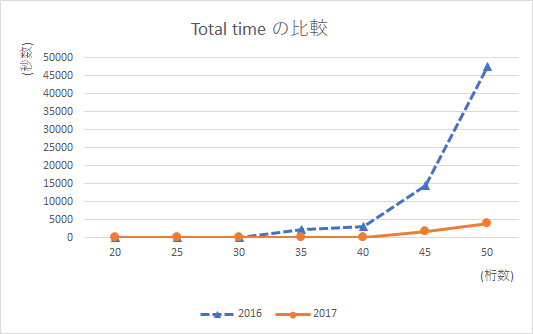
\includegraphics[width=12cm]{Total_time.png}
\end{center}
\caption{プログラム全体の実行にかかった時間}
\label{fig:prog}
\end{figure}

図5.1,図5.2の結果から,Stage2においての計算速度が6~7倍向上したことが分かり,プログラム全体の速度の大幅な改善が確認された.\par

\bunseki{水上敬介}

\chapter{まとめ}

\section{前期活動結果}

前期はメンバー全員で楕円曲線法の学習から初め,楕円曲線法の概要を理解した.その後は理論班とプログラム班に分かれた.\par
理論班はBaby-step Giant-step法について理解し,その内容をプログラム班に教えた.また,論文を探して効率の良い曲線についての考察を行った.\par
プログラム班は昨年度のプログラムの解読を行い,省メモリ化,高速化を行なった.また,理論班の説明を受けBaby-step Giant-step法のアルゴリズムの実装を行った.\par

\bunseki{外山拓}

\section{後期の展望}

後期の活動として,理論班は,Baby-step Giant-step法の素数ペアリングの理解,符号付き2進展開やRucus chainを用いたスカラー倍算の理解などが挙げられる.プログラム班は,素数テーブルからの読み出しやスカラー倍算の並列化による高速化の確認が挙げられる.
以上の活動を行い,ECMNET,STUDIO KAMADAへのランクインを目指す.
\bunseki{中島俊平}



\begin{appendix}
%付録の終わり
\end{appendix}


%\backmatter

% 参考文献
\begin{thebibliography}{9}

\bibitem{EN2017}
\newblock ECMNET.
\newblock https://members.loria.fr/PZimmermann/ecmnet/, (最終アクセス 2017年月日)

\bibitem{SK2017}
\newblock STUDIO KAMADA. 
\newblock http://stdkmd.com/, (最終アクセス 2017年月日)

\bibitem{BSGS2006}
\newblock Kris Gaj, Soonhak Kwon, Patrick Baier, Paul Kohlbrenner, Hoang Le, Mohammed Khaleeluddin, Ramakrishna Bachimanchi.
\newblock Implementing the Elliptic Curve Method of Factoring in Reconfigurable Hardware.
\newblock Cryptographic Hardware and Embedded Systems - CHES 2006, 2006

\bibitem{BSGS2017}
\newblock 楕円曲線法(ECM) faireal.net.
\newblock http://www.faireal.net/articles/6/07/, (最終アクセス 2017年月日).

\bibitem{BRENT1986}
\newblock Richard P. Brent.
\newblock Some Integer Factorization Algorithms using Elliptic Curves.
\newblock Australian Computer Science Communications 8 (1986), 149-163

\bibitem{FFT1992}
\newblock Peter Lawrence Montgomery.
\newblock An FFT extension of the elliptic curve method of factorization.
\newblock University of California at Los Angeles Los Angeles, CA, USA, 1992

\bibitem{MONTG1986}
\newblock Peter Lawrence Montgomery.
\newblock Speeding the Pollard and Elliptic Curve Methods of Factorization.
\newblock Mathematics of Computation. 48 (177): 243–264, 1987






\end{thebibliography}

\end{document}